\documentclass[aspectratio=169]{beamer}
% Gantt chart in the style of the example on slide 13 of the introduction:
% plain grid table, filled turquoise cells, milestone arrows above the header.
% To use in the ILIAS template: copy the lines marked "Gantt" and the frame.

\usepackage{tikz}                          % Gantt
\definecolor{ganttfill}{RGB}{0,232,200}    % Gantt (turquoise as in example)
\definecolor{ganttgrid}{RGB}{110,160,200}  % Gantt (light blue grid lines)
\definecolor{ganttbreak}{RGB}{225,225,225} % Gantt (break column)

% ======================= EDIT HERE =======================================
% Column headers. Column numbers used below:
%   1=CW45  2=CW46  3=CW47  4=CW48  5=CW49  6=CW50  7=CW51  8=Break (CW52-53)
%   9=CW1  10=CW2  11=CW3  12=CW4  13=CW5  14=CW6  15=CW7
\def\weeks{CW45,CW46,CW47,CW48,CW49,CW50,CW51,Break,CW1,CW2,CW3,CW4,CW5,CW6,CW7}
\def\nweeks{15}
\def\breakcol{8}   % column drawn grey as holiday break (set 0 to disable)

% Work packages: {label}/{list of filled columns}
\def\packages{%
  {Familiarization}/{1,2},
  {JAX port: Method 1 (reparam.)}/{3,4},
  {JAX port: Method 2 (trust region)}/{3,4},
  {Test functions \& samplers}/{3,4},
  {Runner \& BBOB benchmarks}/{4,5,6},
  {MuJoCo setup \& baseline}/{4,5,6},
  {VO-MPC integration}/{6,7,9},
  {MPC experiments \& comparison}/{9,10,11,12},
  {Report writing}/{12,13,14,15},
  {Presentations}/{1,2,6,7,14,15}}

% Milestones: {label}/{column}/{height level 1 or 2}/{label side}
% The arrow points to the RIGHT edge (= end of week) of the given column.
% Label side: west = label right of arrow, east = label left of arrow.
\def\milestones{%
  {Project presentation}/2/2/west,
  {JAX port validated}/4/1/west,
  {Midterm}/7/2/west,
  {MPC running}/9/1/west,
  {Results frozen}/12/2/east,
  {Final}/15/1/east}

% Geometry
\def\labelw{4.6}   % width of first column (cm)
\def\colw{0.68}    % width of each week column (cm)
\def\rowh{0.36}    % row height (cm)
% =========================================================================

\begin{document}

\begin{frame}{Project Plan}
\centering
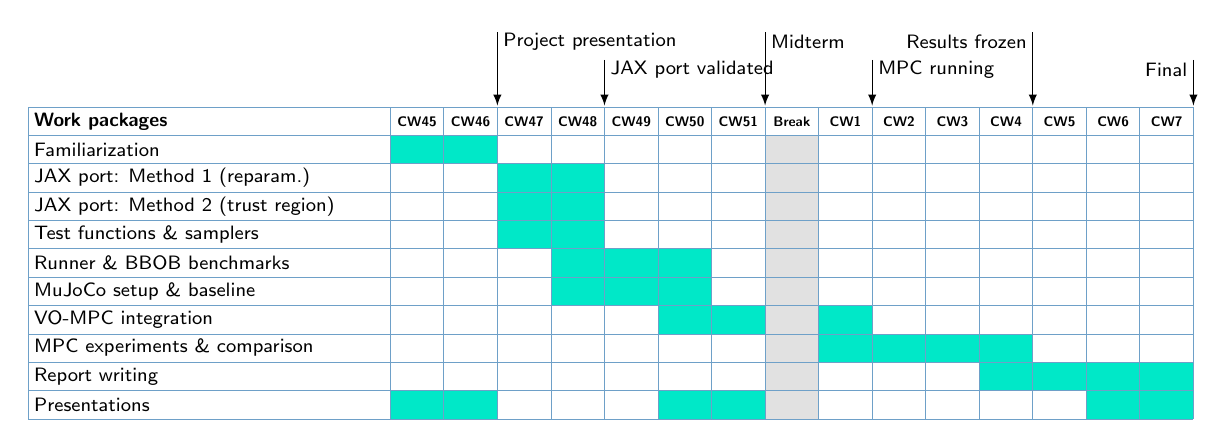
\begin{tikzpicture}[font=\scriptsize\sffamily, x=1cm, y=1cm]
  \foreach \l/\cols [count=\i] in \packages {\xdef\nrows{\i}}
  \pgfmathsetmacro{\W}{\labelw+\nweeks*\colw}
  \pgfmathsetmacro{\H}{(\nrows+1)*\rowh}

  % ---- break column ----
  \ifnum\breakcol>0
    \fill[ganttbreak] ({\labelw+(\breakcol-1)*\colw},{-\rowh}) rectangle
                      ({\labelw+\breakcol*\colw},-\H);
  \fi

  % ---- filled cells + labels ----
  \foreach \l/\cols [count=\i] in \packages {
    \foreach \c in \cols {
      \fill[ganttfill]
        ({\labelw+(\c-1)*\colw},{-(\i+1)*\rowh}) rectangle
        ({\labelw+\c*\colw},{-\i*\rowh});
    }
    \node[anchor=west, inner sep=2pt] at (0,{-(\i+0.5)*\rowh}) {\l};
  }

  % ---- header ----
  \node[anchor=west, inner sep=2pt, font=\scriptsize\sffamily\bfseries]
    at (0,{-0.5*\rowh}) {Work packages};
  \foreach \w [count=\j] in \weeks {
    \node[font=\tiny\sffamily\bfseries] at ({\labelw+(\j-0.5)*\colw},{-0.5*\rowh}) {\w};
  }

  % ---- grid ----
  \foreach \r in {0,...,\nrows} {
    \draw[ganttgrid, line width=0.3pt] (0,{-\r*\rowh}) -- (\W,{-\r*\rowh});
  }
  \draw[ganttgrid, line width=0.3pt] (0,-\H) -- (\W,-\H);
  \draw[ganttgrid, line width=0.3pt] (0,0) -- (0,-\H);
  \foreach \c in {0,...,\nweeks} {
    \draw[ganttgrid, line width=0.3pt] ({\labelw+\c*\colw},0) -- ({\labelw+\c*\colw},-\H);
  }

  % ---- milestones: arrow onto the end of the given week ----
  \foreach \m/\c/\lv/\side in \milestones {
    \pgfmathsetmacro{\top}{0.25+0.35*\lv}
    \draw[-latex, line width=0.4pt] ({\labelw+\c*\colw},\top) -- ({\labelw+\c*\colw},0.02);
    \node[anchor=\side, inner sep=2pt] at ({\labelw+\c*\colw},{\top-0.12}) {\m};
  }
\end{tikzpicture}

\vspace{0.4em}
{\tiny Break: Christmas holidays (CW 52--53). Arrows mark the end of the week.}
\end{frame}

\end{document}